\documentclass{beamer}
\usetheme{Madrid}
\usecolortheme{default}

% Slimming down the footer to save space and remove the date bar
\setbeamertemplate{footline}[frame number]
\setbeamertemplate{navigation symbols}{}

\usepackage[utf8]{inputenc}
\usepackage{graphicx}
\usepackage{tikz}
\usetikzlibrary{shapes,arrows,positioning,fit,backgrounds}
\usepackage{listings}
\usepackage{algorithm}
\usepackage{algpseudocode}
\usepackage{pdflscape}
\usepackage{amsmath}

% Path to images (relative to this file)
\graphicspath{{./images/}}

\title[EHR: Pharmacy Module]{Electronic Health Record: Pharmacy Organization Module}
\subtitle{Enterprise-Grade Platform Using Hyperledger Fabric and Docker Swarm}
\author[Ankit, Mohit, Ronit]{
    ANKIT CHAUDHARI (25CSM2R03) \\
    MOHIT TOMAR (25CSM2R13) \\
    RONITSINGH RAWAT (25CSM2S06)
}
\institute[NITW]{
    Under the guidance of \textbf{PROF. ERUKALA SURESH BABU} \\
    \vspace{10pt}
    DEPARTMENT OF COMPUTER SCIENCE AND ENGINEERING \\
    NATIONAL INSTITUTE OF TECHNOLOGY WARANGAL
}
\date{April, 2026}

\begin{document}

\begin{frame}
    \titlepage
\end{frame}

\begin{frame}{Outline}
    \tableofcontents
\end{frame}

\section{Introduction}
\begin{frame}{Abstract}
    The Electronic Health Record (EHR) System is a decentralized, secure, and scalable platform designed for pharmaceutical inventory and patient record management.
    \begin{itemize}
        \item \textbf{Decentralization:} Built on Hyperledger Fabric.
        \item \textbf{Privacy:} Attribute-Based Access Control (ABAC).
        \item \textbf{Scalability:} Docker Swarm orchestration across multiple nodes.
        \item \textbf{Hybrid Storage:} On-chain metadata and off-chain IPFS document storage.
    \end{itemize}
\end{frame}

\section{System Architecture}
\begin{frame}{High-Level Architecture}
    \centering
    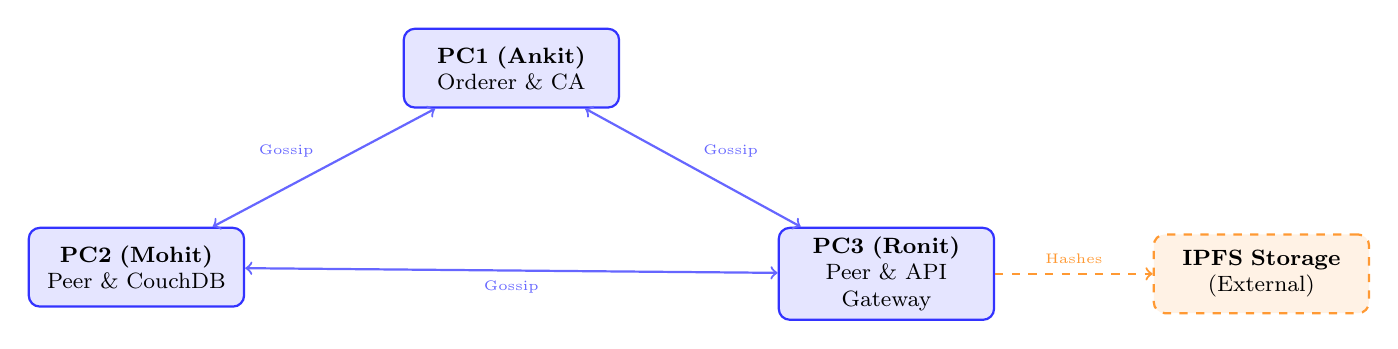
\begin{tikzpicture}[
        node distance=1.5cm and 2cm,
        box/.style={draw=blue!80, fill=blue!10, text width=2.5cm, align=center, minimum height=1cm, rounded corners, thick, font=\footnotesize},
        ext/.style={draw=orange!80, fill=orange!10, text width=2.5cm, align=center, minimum height=1cm, rounded corners, thick, dashed, font=\footnotesize}
    ]
        
        \node[box] (pc1) {\textbf{PC1 (Ankit)}\\Orderer \& CA};
        \node[box, below left=of pc1] (pc2) {\textbf{PC2 (Mohit)}\\Peer \& CouchDB};
        \node[box, below right=of pc1] (pc3) {\textbf{PC3 (Ronit)}\\Peer \& API Gateway};
        
        \node[ext, right=2cm of pc3] (ipfs) {\textbf{IPFS Storage}\\(External)};
        
        \draw[<->, thick, blue!60] (pc1) -- node[above left, font=\tiny] {Gossip} (pc2);
        \draw[<->, thick, blue!60] (pc1) -- node[above right, font=\tiny] {Gossip} (pc3);
        \draw[<->, thick, blue!60] (pc2) -- node[below, font=\tiny] {Gossip} (pc3);
        
        \draw[->, thick, dashed, orange!80] (pc3) -- node[above, font=\tiny] {Hashes} (ipfs);
        
    \end{tikzpicture}
    \vspace{10pt}
    \begin{itemize}
        \item Layered Tiers: Presentation, Application, Blockchain, Storage.
        \item Distributed over 3 physical machines via Tailscale VPN.
    \end{itemize}
\end{frame}

\begin{frame}{Transaction Flow: Write Operation}
    \centering
    \scalebox{0.55}{
    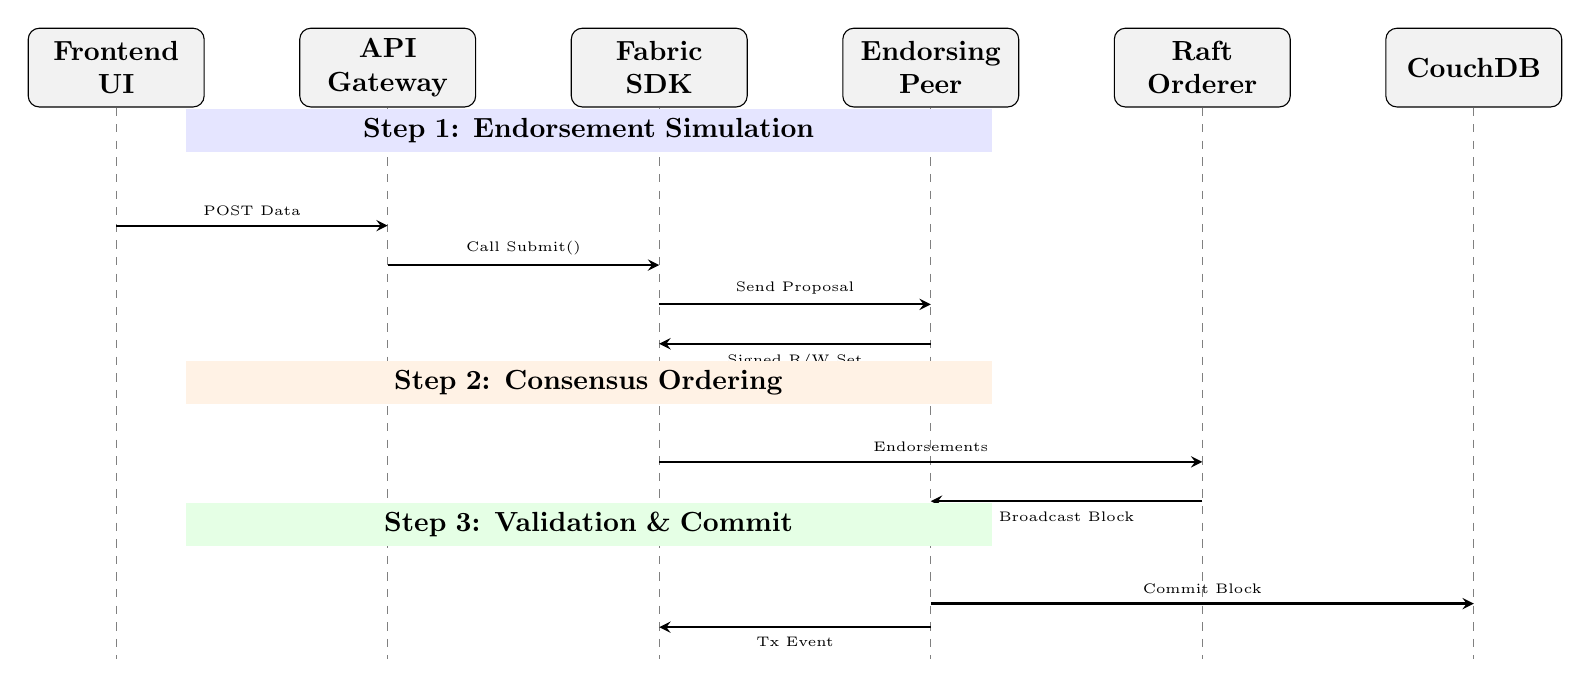
\begin{tikzpicture}[
        node distance=1.2cm,
        actor/.style={draw, fill=gray!10, text width=2cm, align=center, minimum height=1cm, rounded corners},
        arrow/.style={->, thick, >=stealth}
    ]
        \node[actor] (UI) {\textbf{Frontend UI}};
        \node[actor, right=of UI] (API) {\textbf{API Gateway}};
        \node[actor, right=of API] (SDK) {\textbf{Fabric SDK}};
        \node[actor, right=of SDK] (Peer) {\textbf{Endorsing Peer}};
        \node[actor, right=of Peer] (Orderer) {\textbf{Raft Orderer}};
        \node[actor, right=of Orderer] (DB) {\textbf{CouchDB}};

        \foreach \i in {UI, API, SDK, Peer, Orderer, DB} {
            \draw[dashed, gray] (\i.south) -- ++(0,-7);
        }
        
        \node[fill=blue!10, text width=10cm, align=center] at (6,-0.8) {\textbf{Step 1: Endorsement Simulation}};
        \draw[arrow] ([yshift=-1.5cm]UI.south) -- node[above, font=\tiny] {POST Data} ([yshift=-1.5cm]API.south);
        \draw[arrow] ([yshift=-2.0cm]API.south) -- node[above, font=\tiny] {Call Submit()} ([yshift=-2.0cm]SDK.south);
        \draw[arrow] ([yshift=-2.5cm]SDK.south) -- node[above, font=\tiny] {Send Proposal} ([yshift=-2.5cm]Peer.south);
        \draw[arrow] ([yshift=-3.0cm]Peer.south) -- node[below, font=\tiny] {Signed R/W Set} ([yshift=-3.0cm]SDK.south);
        
        \node[fill=orange!10, text width=10cm, align=center] at (6,-4.0) {\textbf{Step 2: Consensus Ordering}};
        \draw[arrow] ([yshift=-4.5cm]SDK.south) -- node[above, font=\tiny] {Endorsements} ([yshift=-4.5cm]Orderer.south);
        \draw[arrow] ([yshift=-5.0cm]Orderer.south) -- node[below, font=\tiny] {Broadcast Block} ([yshift=-5.0cm]Peer.south);

        \node[fill=green!10, text width=10cm, align=center] at (6,-5.8) {\textbf{Step 3: Validation \& Commit}};
        \draw[arrow] ([yshift=-6.3cm]Peer.south) -- node[above, font=\tiny] {Commit Block} ([yshift=-6.3cm]DB.south);
        \draw[arrow] ([yshift=-6.6cm]Peer.south) -- node[below, font=\tiny] {Tx Event} ([yshift=-6.6cm]SDK.south);
    \end{tikzpicture}
    }
\end{frame}

\section{Individual Contributions}

% --- ANKIT ---
\subsection{Ankit Chaudhari}
\begin{frame}{Infrastructure Architect: Ankit Chaudhari (25CSM2R03)}
    \begin{block}{Role \& Responsibility}
        Responsible for core network infrastructure, Docker Swarm orchestration, and the Manager Governance Portal.
    \end{block}
    \begin{itemize}
        \item \textbf{Containers Hosted on PC1:} Fabric CA, Raft Orderer, Peer0, CouchDB0, Manager Portal.
        \item \textbf{Key Highlights:} Automated \texttt{deploy.sh} script, MSP distribution via SCP, and Network Health Monitoring.
    \end{itemize}
\end{frame}

\begin{frame}{Manager Dashboard (Ankit Chaudhari - 25CSM2R03)}
    \centering
    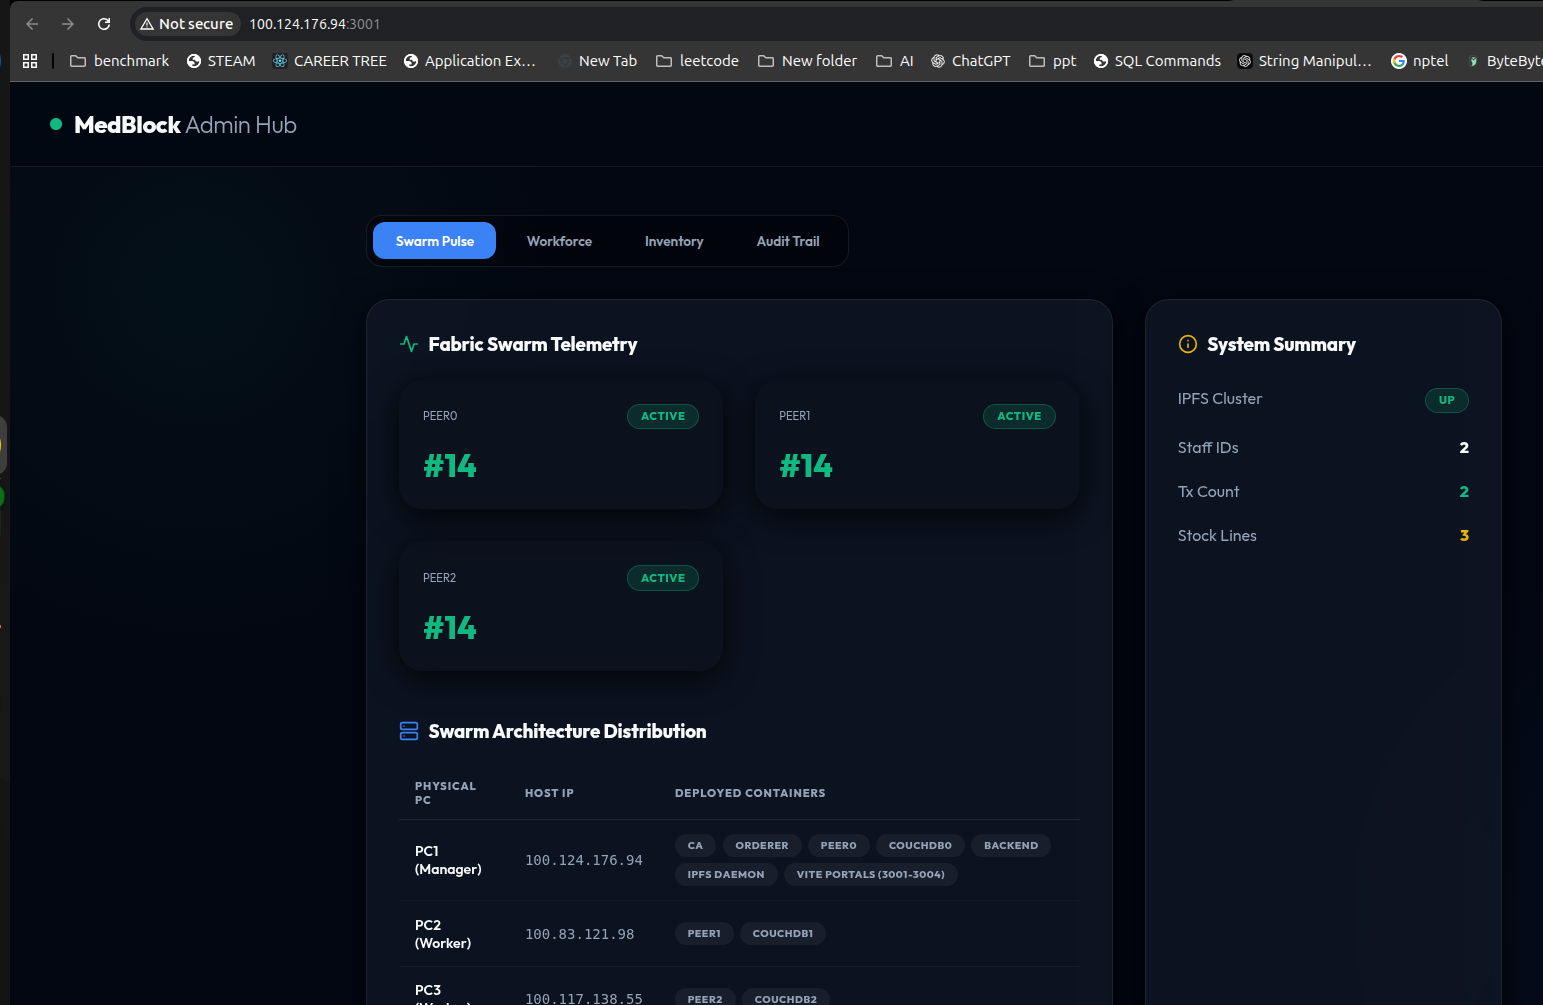
\includegraphics[width=0.9\textwidth,height=0.55\textheight,keepaspectratio]{dash-board.png}
    \begin{itemize}
        \item \textbf{Description:} A high-level governance interface allowing hospital administrators to seamlessly oversee all interconnected system modules, evaluate real-time API gateways, and monitor global network health metrics.
    \end{itemize}
    \vfill {\footnotesize \hfill \textbf{Contribution by: Ankit Chaudhari (25CSM2R03)}}
\end{frame}

\begin{frame}{Workforce Registry (Ankit Chaudhari - 25CSM2R03)}
    \centering
    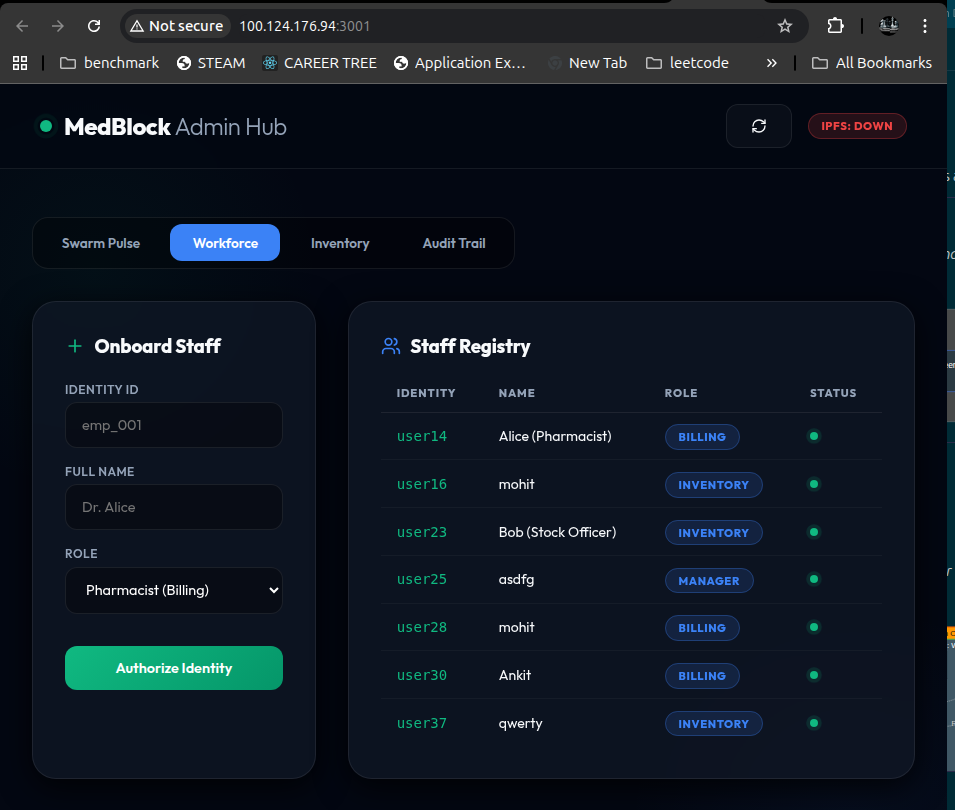
\includegraphics[width=0.9\textwidth,height=0.55\textheight,keepaspectratio]{workforce.png}
    \begin{itemize}
        \item \textbf{Description:} The primary employee enrollment interface. It securely assigns specific ABAC roles (Doctor, Pharmacist, Inventory) and automatically provisions deterministic cryptographic X.509 identities via the Fabric CA.
    \end{itemize}
    \vfill {\footnotesize \hfill \textbf{Contribution by: Ankit Chaudhari (25CSM2R03)}}
\end{frame}

\begin{frame}{Network Monitoring (Ankit Chaudhari - 25CSM2R03)}
    \centering
    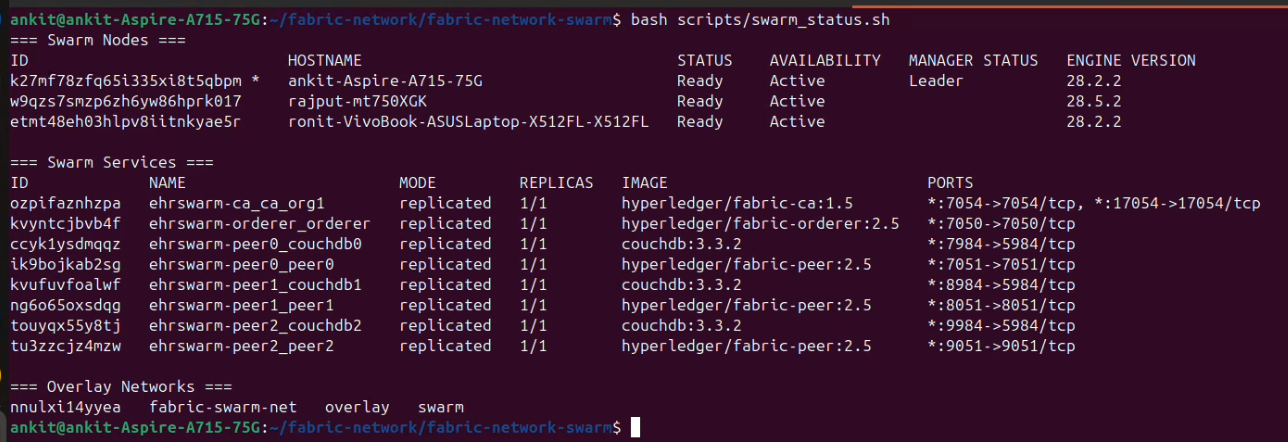
\includegraphics[width=0.9\textwidth,height=0.55\textheight,keepaspectratio]{status.png}
    \begin{itemize}
        \item \textbf{Description:} Provides real-time graphical visualization of overall Swarm node availability, current ledger block height across physical machines, and reliable Gossip data synchronization status.
    \end{itemize}
    \vfill {\footnotesize \hfill \textbf{Contribution by: Ankit Chaudhari (25CSM2R03)}}
\end{frame}

\begin{frame}{Blockchain Audit Trail (Ankit Chaudhari - 25CSM2R03)}
    \centering
    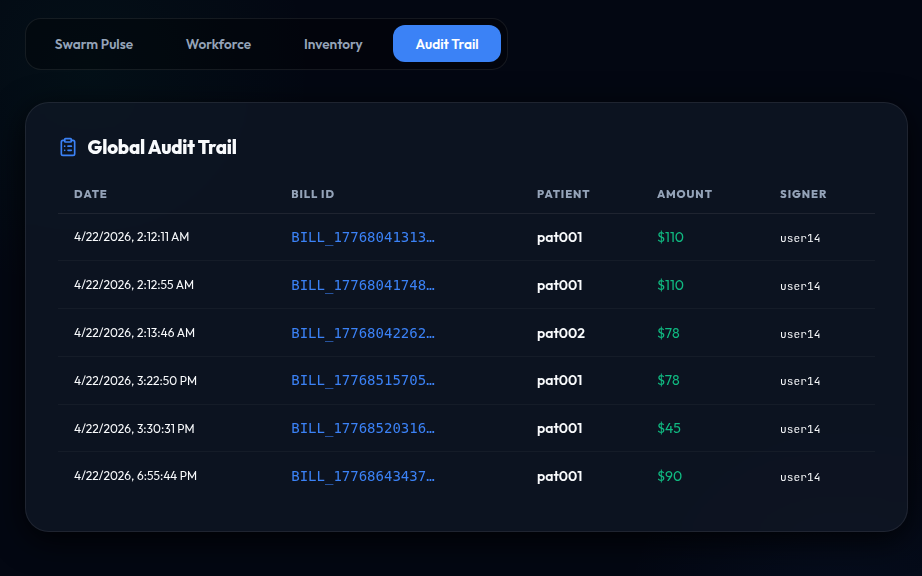
\includegraphics[width=0.9\textwidth,height=0.55\textheight,keepaspectratio]{audit.png}
    \begin{itemize}
        \item \textbf{Description:} An immutable and transparent record of all historical activities recorded on the ledger, effectively allowing hospital managers to easily pull global hospital records for comprehensive auditing and oversight.
    \end{itemize}
    \vfill {\footnotesize \hfill \textbf{Contribution by: Ankit Chaudhari (25CSM2R03)}}
\end{frame}

\begin{frame}{Inventory Oversight (Ankit Chaudhari - 25CSM2R03)}
    \centering
    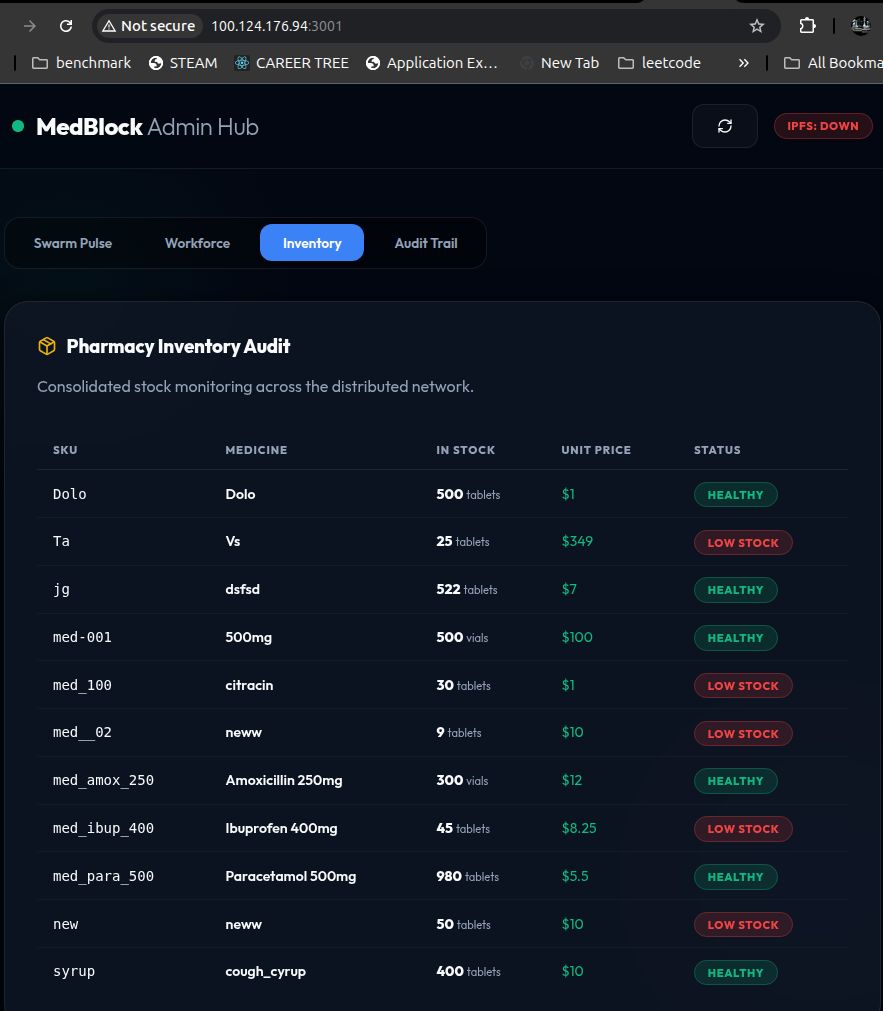
\includegraphics[width=0.9\textwidth,height=0.55\textheight,keepaspectratio]{inventory.png}
    \begin{itemize}
        \item \textbf{Description:} A specifically assigned read-only global oversight interface showing real-time medicine stock levels aggregated across all pharmaceutical points, seamlessly ensuring total transparency in supply.
    \end{itemize}
    \vfill {\footnotesize \hfill \textbf{Contribution by: Ankit Chaudhari (25CSM2R03)}}
\end{frame}

% --- MOHIT ---
\subsection{Mohit Tomar}
\begin{frame}{Smart Contract Lead: Mohit Tomar (25CSM2R13)}
    \begin{block}{Role \& Responsibility}
        Development of Node.js Chaincode, CouchDB Rich Queries, and clinical portals (Patient \& Pharmacist).
    \end{block}
    \begin{itemize}
        \item \textbf{Containers Hosted on PC2:} Peer1, CouchDB1, Patient Portal, Pharmacist Portal.
        \item \textbf{Key Highlights:} Identity Resolution algorithm, attribute-based access control, and IPFS anchoring logic.
    \end{itemize}
\end{frame}

\begin{frame}{Patient Portal (Part 1)}
    \centering
    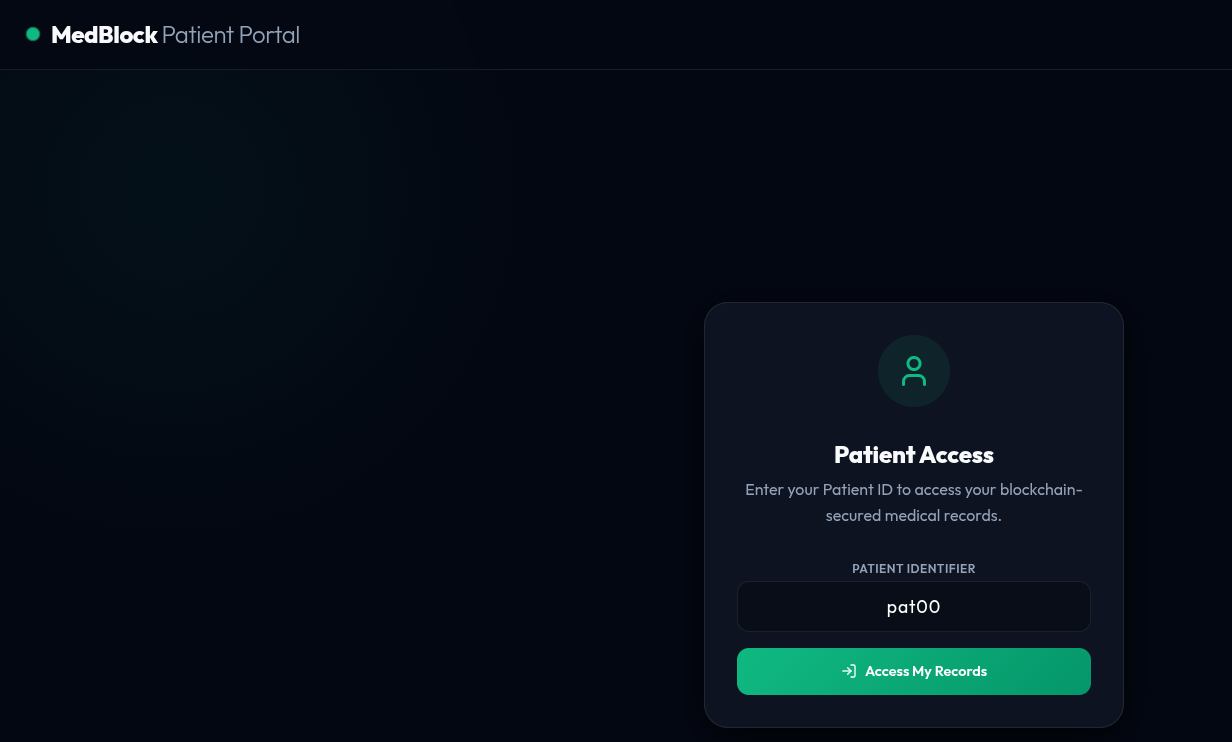
\includegraphics[width=0.9\textwidth,height=0.55\textheight,keepaspectratio]{patient_portal1.png}
    \begin{itemize}
        \item \textbf{Description:} The core Self-Sovereign Identity (SSI) portal demonstrating patient access. The dashboard gives the patient a clear, chronological overview of their complete medical history logged safely onto the ledger.
    \end{itemize}
    \vfill {\footnotesize \hfill \textbf{Contribution by: Mohit Tomar (25CSM2R13)}}
\end{frame}

\begin{frame}{Patient Portal (Part 2)}
    \centering
    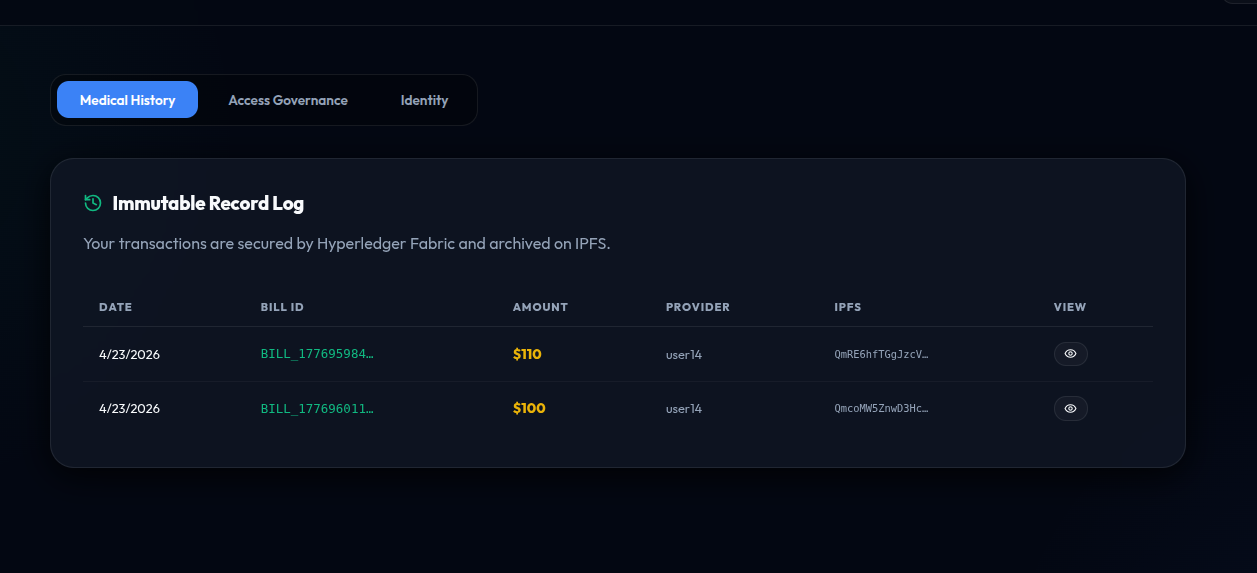
\includegraphics[width=0.9\textwidth,height=0.55\textheight,keepaspectratio]{patient_portal2.png}
    \begin{itemize}
        \item \textbf{Description:} Features decentralized off-chain IPFS document storage integration holding heavy medical reports, allowing patients to explicitly grant or revoke viewing rights selectively.
    \end{itemize}
    \vfill {\footnotesize \hfill \textbf{Contribution by: Mohit Tomar (25CSM2R13)}}
\end{frame}

\begin{frame}{Pharmacist Portal (Part 1)}
    \centering
    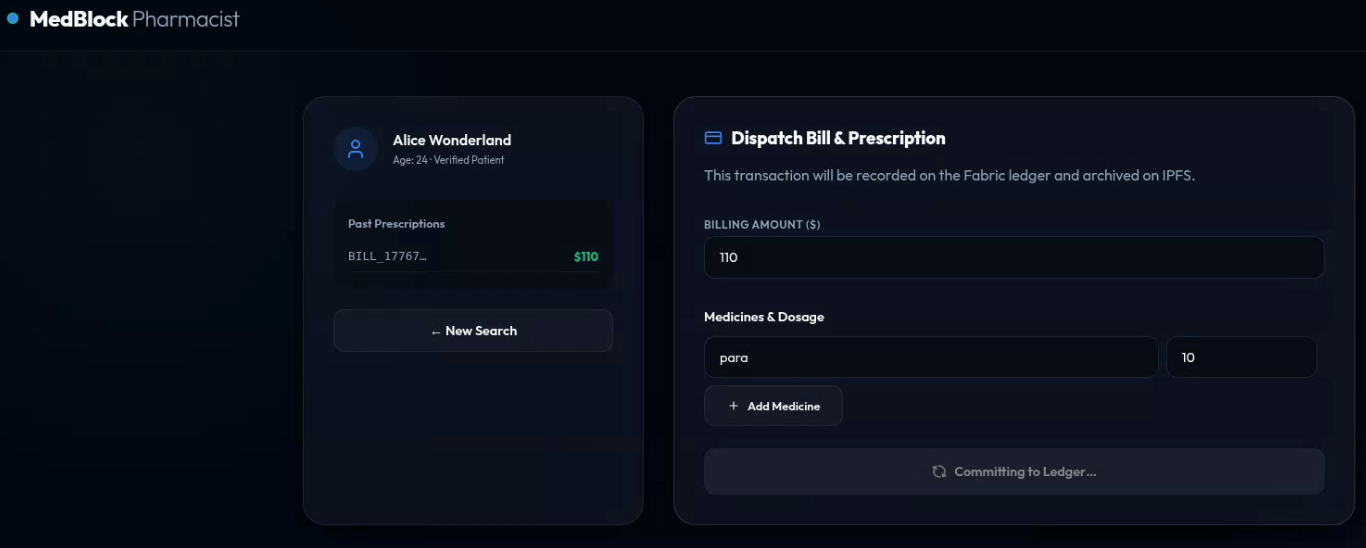
\includegraphics[width=0.9\textwidth,height=0.55\textheight,keepaspectratio]{pharma_portal1.png}
    \begin{itemize}
        \item \textbf{Description:} A dedicated pharmacy billing interface operating purely on Attribute-Based Access Control (ABAC) principles, strictly limiting the pharmacist's view only to prescribed medications on demand.
    \end{itemize}
    \vfill {\footnotesize \hfill \textbf{Contribution by: Mohit Tomar (25CSM2R13)}}
\end{frame}

\begin{frame}{Pharmacist Portal (Part 2)}
    \centering
    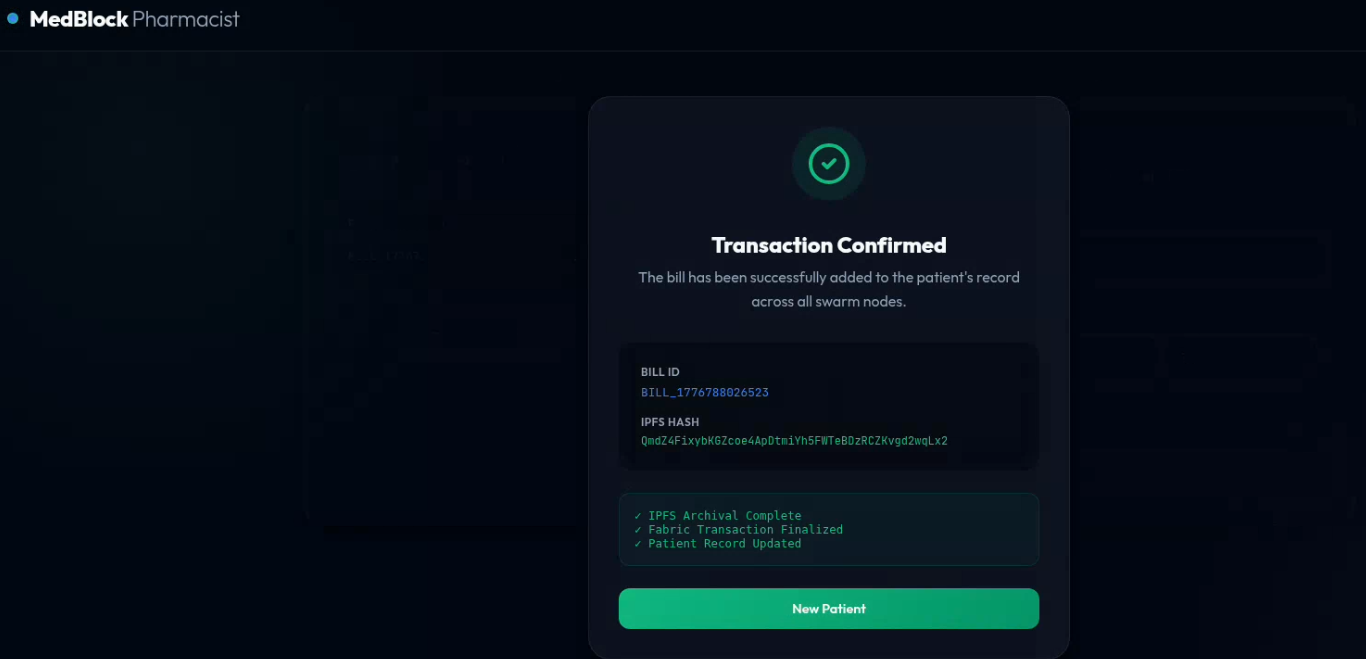
\includegraphics[width=0.9\textwidth,height=0.55\textheight,keepaspectratio]{pharma_portal2.png}
    \begin{itemize}
        \item \textbf{Description:} Seamlessly tracks prescription fulfillment and features dynamic integration with the global supply chain ledger, allowing instant atomic updates bridging the billing flow and physical stock count.
    \end{itemize}
    \vfill {\footnotesize \hfill \textbf{Contribution by: Mohit Tomar (25CSM2R13)}}
\end{frame}

% --- RONIT ---
\subsection{Ronitsingh Rawat}
\begin{frame}{API Gateway Architect: Ronitsingh Rawat (25CSM2S06)}
    \begin{block}{Role \& Responsibility}
        Central API Gateway (Node.js SDK), Wallet Management, and Inventory Supply Chain Application.
    \end{block}
    \begin{itemize}
        \item \textbf{Containers Hosted on PC3:} Peer2 (Redundancy), CouchDB2, API Gateway, Inventory Portal.
        \item \textbf{Key Highlights:} Smart Routing algorithm, deterministic certificate mapping, and high availability setup.
    \end{itemize}
\end{frame}

\begin{frame}{State Mirroring: CouchDB2 Interface}
    \centering
    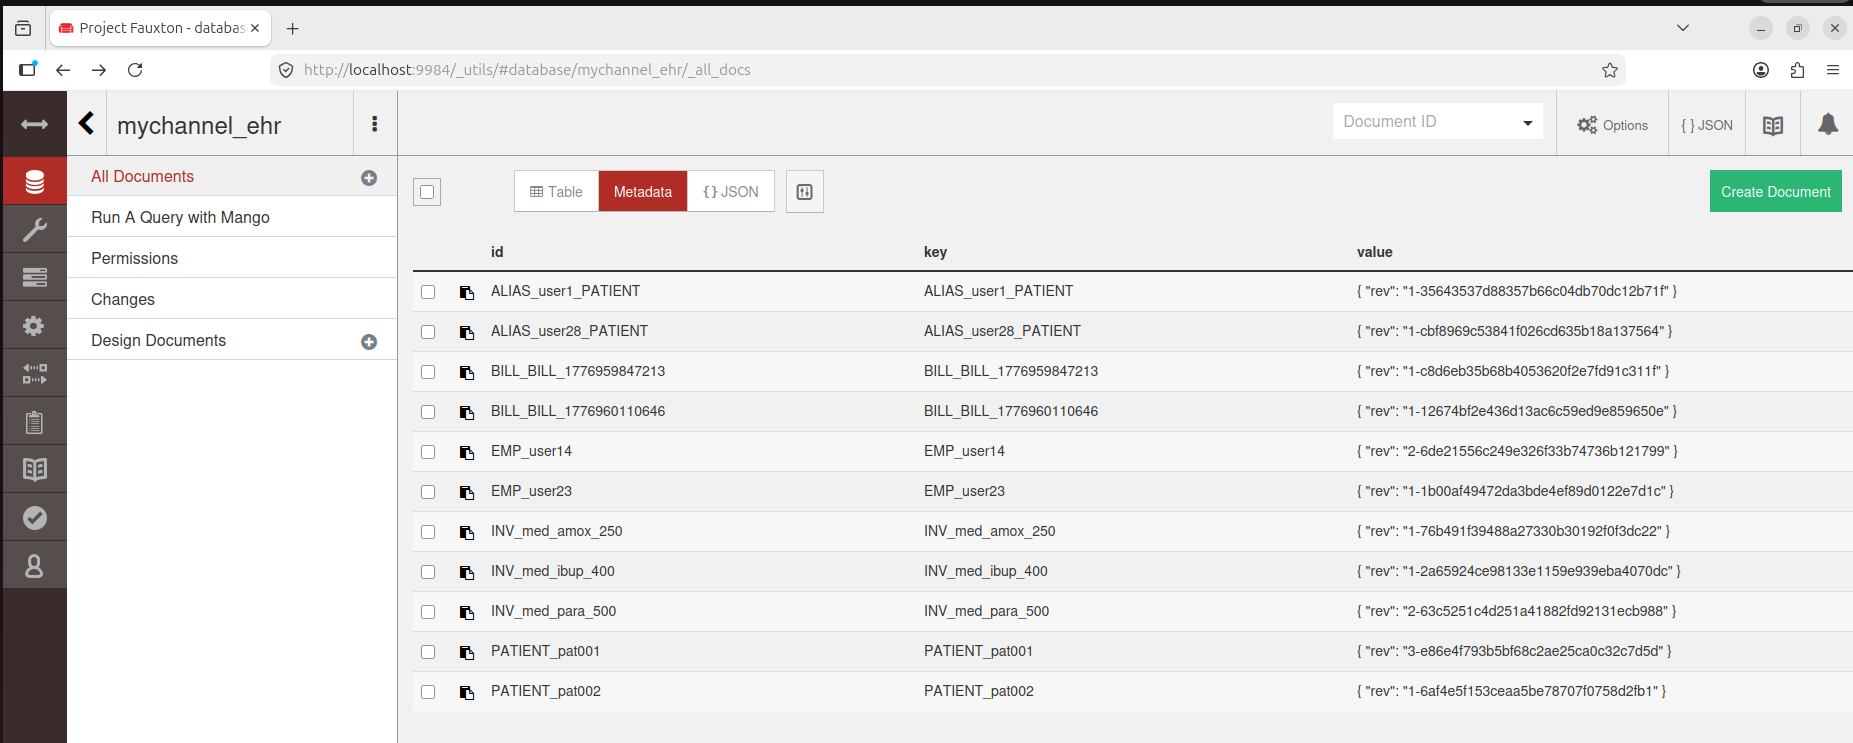
\includegraphics[width=0.9\textwidth,height=0.55\textheight,keepaspectratio]{couchdb.png}
    \begin{itemize}
        \item \textbf{Description:} A live backend look at CouchDB world state mirroring, effectively proving perfect decentralized cross-node data availability, rich JSON querying capabilities, and consensus fidelity across the Swarm.
    \end{itemize}
    \vfill {\footnotesize \hfill \textbf{Contribution by: Ronitsingh Rawat (25CSM2S06)}}
\end{frame}

\begin{frame}{Inventory Supply Chain (Part 1)}
    \centering
    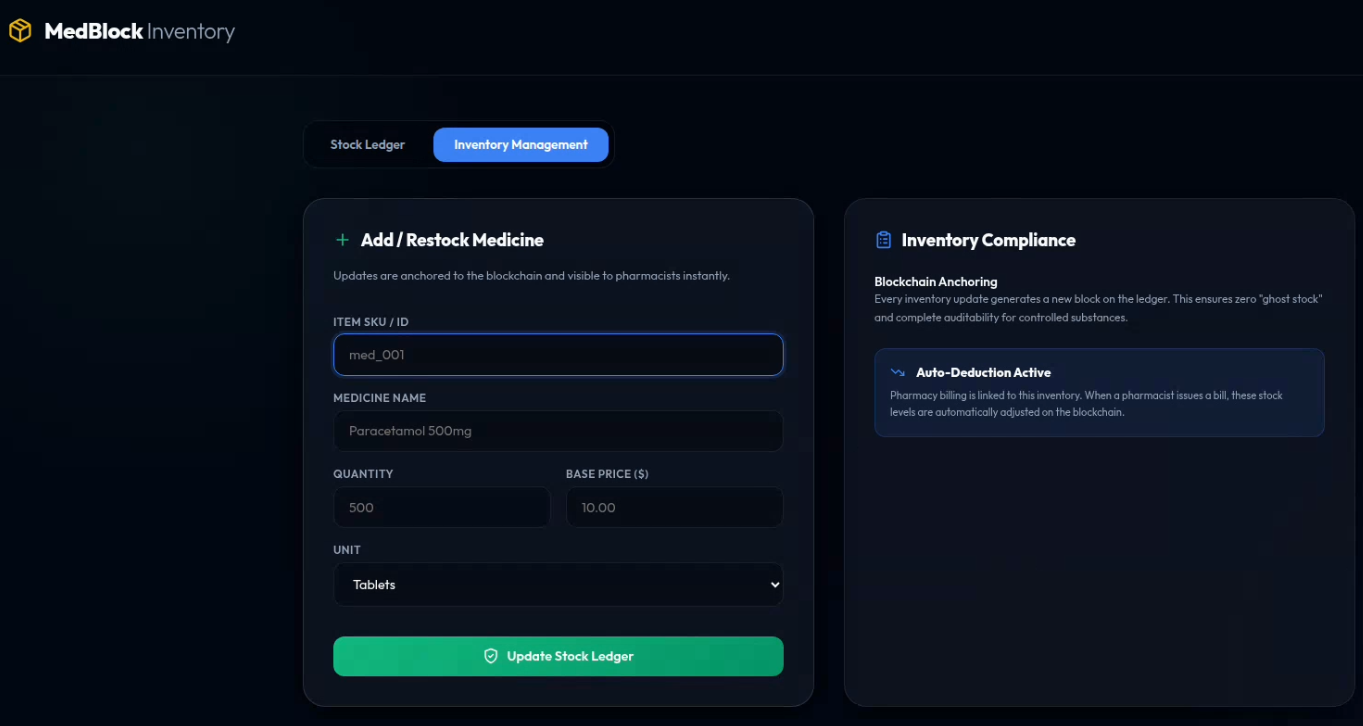
\includegraphics[width=0.9\textwidth,height=0.55\textheight,keepaspectratio]{inventory1.png}
    \begin{itemize}
        \item \textbf{Description:} The primary entry point interface effectively responsible for smoothly adding bulk new medicine stock imports into the blockchain ledger, mathematically tied to irreversible, immutable timestamps.
    \end{itemize}
    \vfill {\footnotesize \hfill \textbf{Contribution by: Ronitsingh Rawat (25CSM2S06)}}
\end{frame}

\begin{frame}{Stock Management (Part 2)}
    \centering
    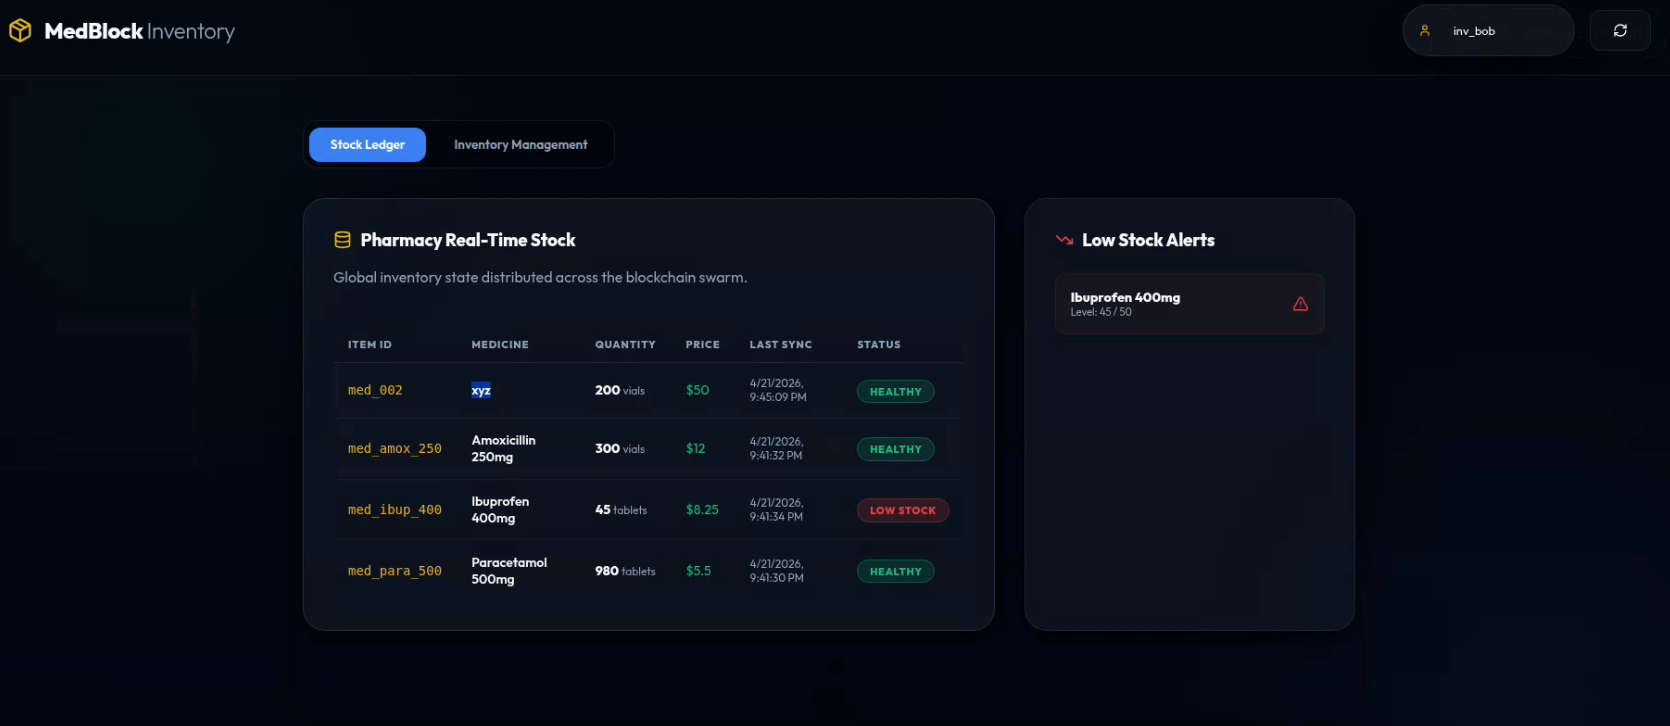
\includegraphics[width=0.9\textwidth,height=0.55\textheight,keepaspectratio]{inventory2.png}
    \begin{itemize}
        \item \textbf{Description:} Comprehensive visual list view managing all existing inventoried stocks and tracking automated ledger deductions, securely linked atomically to successful pharmacy billing transactions across the platform.
    \end{itemize}
    \vfill {\footnotesize \hfill \textbf{Contribution by: Ronitsingh Rawat (25CSM2S06)}}
\end{frame}

\section{Verification}
\begin{frame}{Network Verification}
    \begin{itemize}
        \item \textbf{Ledger Sync:} All three peers (Peer0, Peer1, Peer2) reported identical block heights and matching hash values.
        \item \textbf{State Replication:} CouchDB instances on all nodes show synchronized world state.
        \item \textbf{Fault Tolerance:} Verified by taking one peer offline (PC2) and routing transactions through the redundant node (PC3).
    \end{itemize}
\end{frame}

\section{Conclusion}
\begin{frame}{Conclusion}
    \begin{enumerate}
        \item Successfully implemented a distributed EHR system across multiple physical nodes.
        \item Achieved perfect data consistency via Hyperledger Fabric's Gossip protocol.
        \item Ensured security and privacy through ABAC and X.509 digital identities.
        \item Built functional clinical, administrative, and inventory portals.
    \end{enumerate}
\end{frame}

\begin{frame}{Future Work}
    \begin{itemize}
        \item \textbf{AI/ML Integration:} Implementing predictive analytics for hospital inventory resupply based on historical prescription rates.
        \item \textbf{Cross-Hospital Interoperability:} Expanding the channel configuration to allow external hospital organizations to query authorized records securely.
        \item \textbf{Mobile Application:} Developing dedicated native mobile applications for the Patient and Pharmacist portals for improved accessibility.
    \end{itemize}
\end{frame}

\begin{frame}
    \centering
    \Huge Thank You! \\
    \vspace{20pt}
    \Large Questions?
\end{frame}

\end{document}
